\documentclass{beamer}

\usepackage[T1]{fontenc}
\usepackage[utf8]{inputenc}
\usepackage[english]{babel}
\usepackage{lmodern}
\usepackage{listings}
% Use Unipd as theme, with options:
% - pageofpages: define the separation symbol of the footer page of pages (e.g.: of, di, /, default: of)
% - logo: position another logo near the Unipd logo in the title page (e.g. department logo), passing the second logo path as option 
% Use the environment lastframe to add the endframe text
%\usetheme[pageofpages=of, logo=dm_logo.png]{Unipd}
\usetheme[pageofpages=of]{Unipd}

\title{Runtimes for Concurrency and Distribution}
\subtitle{Project: Exploration of orchestration challenges in a microservice-based application}
\author{Luca Marchiori}
\date{June 2024}

\lstdefinestyle{mystyle}{
    basicstyle=\ttfamily\tiny,
    breakatwhitespace=false,         
    breaklines=true,                 
    captionpos=b,                    
    keepspaces=true,                 
    showspaces=false,                
    showstringspaces=false,
    showtabs=false,                  
    tabsize=1,
	aboveskip=5pt, % set the space above the lstlisting block
	belowskip=5pt, % set the space below the lstlisting block
}
\lstset{style=mystyle}


\begin{document}

\maketitle

\begin{frame}{Outline}
	\tableofcontents
\end{frame}


\section{Report corrections}


\begin{frame}{Missing notions}
	After reading the comments, I realized that I missed some notions in the report:
	\begin{itemize}
		\item Theoretical definitions (Microservices, REST, ...)
		\item Tool descriptions (Swagger, OpenAPI, RabbitMQ, ...)
		\item Components behavior (Nodeport, Ingress, ...)
	\end{itemize}
		
	In the earliest version of the report I included these sections, but I had to cut them to respect the 10 pages limit.
	\newline
	\newline
	As a technical report, I focused more on explaining the project itself and the implementation details.
\end{frame}


\begin{frame}
	\begin{center}
		\huge{My responses to the "B" comments}
	\end{center}
\end{frame}

\begin{frame}{The "basic" microservices choice}
	\label{common_ms}
	\begin{block}{}
		Why implementing common and basic microservices such as users, auth, and notifications?
	\end{block}
	\begin{itemize}
		\item The goal was to learn more about orchestration, not to develop impressive features.
		\item I didn't want to lose time by thinking of exceptional use cases.
		\item Those are component that I could find in any future project.
	\end{itemize}
	That's why I decided to implement the first basic microservices that came to my mind. 
\end{frame}

\begin{frame}{The "basic" microservices choice}
	The results of my approach:
	\begin{itemize}
		\item I focused more on the orchestration challenges and less on the toy examples.
		\item By dealing with a business domain that is easy to understand I kept a good progress pace.
		\item I could choose the next components to implement not based on the examples but on the area of interest that I wanted to explore.
	\end{itemize}
\end{frame}

\begin{frame}{The exploratory approach}
	I preferred an exploratory approach to get a basic understanding of multiple components of the microservice architecture.
	\newline \newline
	I could dive deep into a smaller number of components, but I would have missed the opportunity to have a global view of the system.
\end{frame}

\begin{frame}{The HPA problem}
The Horizontal Pod Autoscaler (HPA) was not working as expected: Pods were not scaling up when multiple requests were sent to the service.
\begin{block}{}
	\textbf{My mistake:} I stopped looking for a solution after the first assumption that made sense to me.
\end{block}
New debugging session:
\begin{figure}
	\centering
	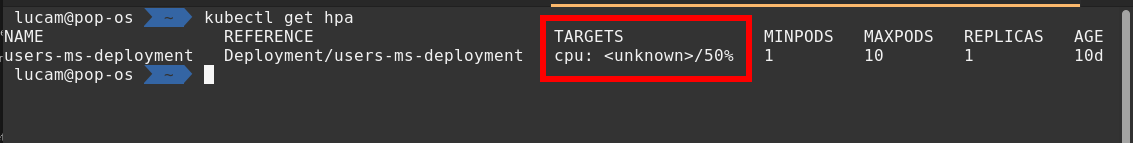
\includegraphics[width=1\linewidth]{./images/hpaProblem.png}
\end{figure}
Something seems to be wrong with the metrics-server. The HPA is not able to retrieve the metrics from the metrics-server.
\end{frame}

\begin{frame}[fragile]{The HPA problem}
Checking with the HPA logs:
	\begin{lstlisting}{language=bash}
		horizontal-pod-autoscaler: failed to get cpu utilization: unable to get metrics for resource cpu: no metrics returned from resource metrics API
		horizontal-pod-autoscaler: invalid metrics (1 invalid out of 1), first error is: failed to get cpu resource metric value: failed to get cpu utilization: unable to get metrics for resource cpu: no metrics returned from resource metrics API
	\end{lstlisting}

	\begin{block}{}
		Problem identified: the metrics-server is not able to retrieve the metrics from the pods.
	\end{block}
\end{frame}

\begin{frame}[fragile]{The HPA problem}
	After some debugging sessions, I found the problems:
	\begin{itemize}
		\item Minikube needs to be started with "--extra-config=kubelet.housekeeping-interval=10s" to avoid caching issues with the metrics-server.
		\item Missing configuration in the users-ms deployment for specifying the resource requests and limits.
	\end{itemize}

	Furthermore, instead of deploying the metrics-server from command line, I moved its deployment to a separate file to better manage the configuration.
\end{frame}

\begin{frame}[fragile]{The HPA problem}
	\begin{figure}
		\centering
		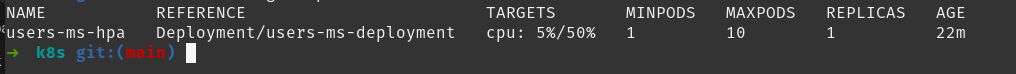
\includegraphics[width=1\linewidth]{./images/hpaFix1.png}
	\end{figure}
	After starting the load test again, the HPA was able to scale up the pods as expected.
	\begin{figure}
		\centering
		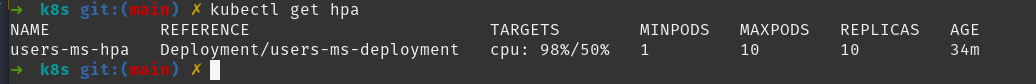
\includegraphics[width=1\linewidth]{./images/hpaFix3.png}
	\end{figure}
	Minikube limitation: no matter the number of pods, the host CPU is the same, so the performance is limited.
\end{frame}
	
\begin{frame}{Updates}
	\textbf{Microservices updates are easy or not?}
	In the report i begin by saying that microservices updates are hard but then I show that they are pretty easy.
	\begin{itemize}
		\item Without orchestration, updates are very challenging.
		\item With Kubernetes are more manageable but still require proper planning.
	\end{itemize}
\end{frame}
\begin{frame}{Updates}
	The "latest" tag leads to:
	\begin{itemize}
		\item Unpredictability
		\item Inconsistent updates
		\item Difficult in debugging and replication
	\end{itemize}
	\begin{block}{}
		Instead, use tags consistent with a version control strategy to ensure stability and traceability.
	\end{block}
	This approach allows for precise control over which image version is deployed, facilitating easier rollbacks and consistent environments across development, testing, and production stages.
\end{frame}

\section{Take-home message}
\begin{frame}{Take-home message}
	% Quale sia, secondo te il principale "take-home message" dell'intera prova d'esame, per un lettore terzo, in relazione ai temi di RCD.
	\begin{block}{}
		Microservices are much more complex than traditional monolithic applications. They require an experienced architectural view because even if tools are available to simplify the orchestration, the complexity of the system requires a deep understanding of the underlying concepts of distributed systems.
	\end{block}
	The decision to implement microservices should be driven by actual needs because it involves completely different skills and organizational structures than traditional applications.
\end{frame}
\section{Learning outcome}
\begin{frame}{Learning outcome}
	% Quale sia stato il tuo personale "learning outcome", per te stesso come studente, rispetto ai temi di RCD da questa prova d'esame.
	These are the key concepts I learned both from the course and the project:
	\begin{itemize}
		% Kubernetes and DOcker and stuff sono molto belli, ma senza una base teorica non si va da nessuna parte. Sento dai miei colleghi che molti li usano perchè vanno di moda ma non sanno realmente cosa stanno facendo.
		\item Tools and technologies are worthless without a clear understanding of the underlying concepts.
		\item Microservices are interesting but the choice of implementing them should be driven by actual needs, not just because they are trendy.
		\item The Asynchronous Communication style enhances decoupling, allows for robust failure handling mechanisms, and offers great scalability support.
	\end{itemize}
\end{frame}

\section{CFU evaluation}
\begin{frame}{CFU evaluation}
	6 CFU equals to 150 hours of work.
	\\
	How I spent my time:
	\begin{itemize}
		\item Lessons: $\sim$ 50 hours
		\item Study: $\sim$ 50 hours
		\item Project: 10 weeks, $\sim$ 6/8 hours per week (60 hours)
	\end{itemize}
	\begin{block}{}
		Good balance between lessons and project, consistent with the CFU assigned.
	\end{block}
\end{frame}

\section{Feedback on the course}
\begin{frame}{Feedback on the course}
	\begin{block}{Good points}
		\begin{itemize}
			\item Very interesting topics that connect basic C.S. concepts with more advanced and real-world applications.
			\item I enjoyed the interactions between the students and the professor, especially for flipped classroom lessons.
		\end{itemize}
	\end{block}
	\begin{block}{Improvements}
		\begin{itemize}
			\item It would have been interesting to have more discussion sessions.
			\item I felt a little lost during the project development. It is hard to start from scratch without a clear idea of what are the expectations.
		\end{itemize}
	\end{block}
\end{frame}

\begin{frame}{Sources of Information}
	\begin{itemize}
		\item \textbf{Official Docker documentation website}
		\begin{itemize}
			\item \url{https://docs.docker.com/}
		\end{itemize}

		\item \textbf{Official Kubernetes documentation website}
		\begin{itemize}
			\item \url{https://kubernetes.io/docs/}
		\end{itemize}

		\item \textbf{Introduction to Microservices}
		\begin{itemize}
			\item \url{https://web.archive.org/web/20240202154248/https://www.nginx.com/blog/introduction-to-microservices/}
		\end{itemize}

		\item \textbf{Building Microservices with Go} - Nic Jackson

		\item \textbf{Building Microservices: Designing Fine-Grained Systems} - Sam Newman

		\item \textbf{Microservices} - Martin Fowler
		\begin{itemize}
			\item \url{https://web.archive.org/web/20180214171522/https://martinfowler.com/articles/microservices.html}
		\end{itemize}
	\end{itemize}
\end{frame}

\setbeamercolor{background canvas}{bg=red_unipd}
\begin{frame}{}
	\begin{center}
		\Huge{\textcolor{white}{Thank you for your attention!}}
	\end{center}
\end{frame}

\setbeamercolor{background canvas}{bg=white}
\begin{frame}{Missing definitions}
	\label{index_1}
	Extra slides for missing definitions:
		\begin{itemize}
			\item \hyperlink{microservices_definitions}{Microservices definitions}
			\item \hyperlink{rest}{REST architectural style}
			\item \hyperlink{swagger_openapi}{What are Swagger and OpenAPI}
			\item \hyperlink{golang}{Why choosing GO as programming language}
		\end{itemize}
\end{frame}


\section{More}
\begin{frame}{Microservices definitions}
	\label{microservices_definitions}
	\begin{block}{}
		“Microservices are \textbf{independently} releasable services that are modeled around a \textbf{business domain}. A service encapsulates functionality and makes it accessible to other services via \textbf{networks}” \footnote{Sam Newman, Building Microservices}
	\end{block}
	\begin{block}{}
		“A microservice is an architectural pattern that arranges an application as a collection of \textbf{loosely coupled}, \textbf{fine-grained services}, communicating through lightweight protocols” \footnote{Martin Fowler, Microservices}
	\end{block}

\hyperlink{index_1}{\beamerbutton{Back to index}}
\end{frame}

\begin{frame}{REST architectural style}
	\begin{block}{}
		REST (Representational State Transfer) is a web architecture style using standard HTTP methods (GET, POST, PUT, DELETE) to interact with resources via URLs.
	\end{block}
	\begin{itemize}
		\item POST: /users (create a new user)
		\item GET: /users/{id} (get a user by id)
		\item GET: /users (get all users)
		\item PUT: /users/{id} (update a user by id)
		\item DELETE: /users/{id} (delete a user by id)
	\end{itemize}
	
	\label{rest}
\hyperlink{index_1}{\beamerbutton{Back to index}}
\end{frame}

\begin{frame}{Why GO as programming language}
	\label{golang}
	\begin{block}{}
		Microservices are language-agnostic, so they can be written in any language as long as they support necessary communication protocols.
		\end{block}
		It is also possible to have different microservices written in different languages as long as they can communicate with each other.
		\newline \newline \newline
		GO was chosen for the project because it has native support for web server making development easier and faster.  \footnote{Thanks to the concurrency features of the language, and the native support for web standards, both Docker and Kubernetes are written in GO.}
\newline
\hyperlink{index_1}{\beamerbutton{Back to index}}
\end{frame}

\begin{frame}{What are Swagger and OpenAPI}
	\label{swagger_openapi}
	\begin{block}{Swagger}
		Swagger is a set of open-source tools built around the OpenAPI Specification that can help in design, build, document and consume REST APIs.
\end{block}
\begin{block}{OpenAPI}
		OpenAPI Specification is a specification for building APIs. It is a language-agnostic specification that describes the structure of REST APIs.
\end{block}
In the project i used OpenAPI to define the API of the application and Swagger to have a GUI for reading the API documentation and test the endpoints.
\newline
\hyperlink{index_1}{\beamerbutton{Back to index}}
\end{frame}

\end{document}
